\input ../SlidePreamble
\input ../preamble

\begin{document}

{\Huge

  \centerline{\bf TTIC 31230, Fundamentals of Deep Learning}
  \bigskip
  \centerline{David McAllester, Winter 2019}

    \vfill
  \centerline{\bf Convolutional Neural Networks (CNNs)}
  \vfill
  \vfill


\slidetwo{What is a CNN?}
{VGG, Zisserman, 2014}

\centerline{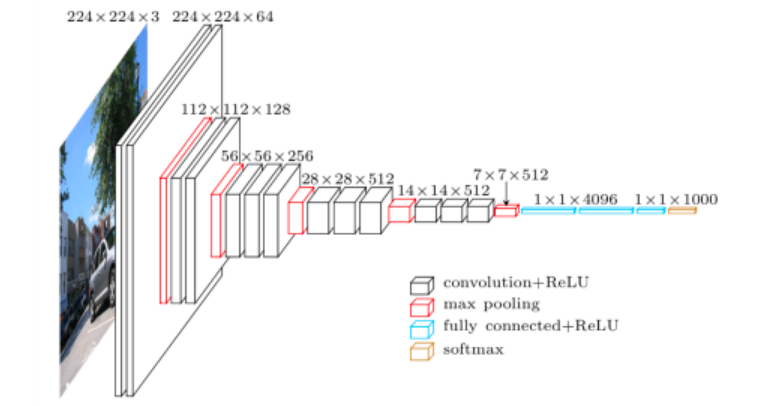
\includegraphics[width = 8.0in]{../images/VGG}}
\centerline{\large Davi Frossard}

\slide{Review: Einstein Notation for Linear Threshold Layer}

$${\color{red} y} = \sigma\left(W{\color{red} x} - B\right)$$

\vfill
is an abbreviation for
\begin{eqnarray*}
  {\color{red} y[b,j]} & = & \sigma\left(\left(\sum_i\;W[j,i] \;{\color{red} x[b,i]}\right) - B[j]\right) 
\end{eqnarray*}

\vfill
Think of this as a separate assignment statement for each {\color{red} $(b,j)$}.

\vfill
Each {\color{red} $y[b,j]$} is the output of a ``linear threshold unit''.

\vfill
Einstein notation makes all indeces and summations explicit.

\slideplain{A Convolution Layer}

\centerline{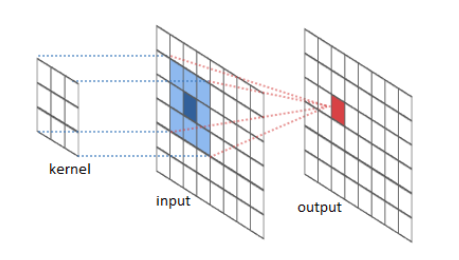
\includegraphics[width = 2.5in]{../images/Convolution}}
\centerline{$W[\Delta x,\Delta y,i,j]$\hspace{6ex}$L_{\mathrm{IN}}[b,x,y,i]$\hspace{6ex}$L_{\mathrm{out}}[b,x,y,j]$}
\centerline{\large River Trail Documentation}

\vfill
{\tt Procedure CONV}$(W[\Delta x, \Delta y, i, j], B[j], L_{\mathrm{in}}[b,x,y,i])$
\begin{eqnarray*}
 & &  \mbox{Return}\;\;L_{\mathrm{out}}[b,x,y,j] \\
 & = &   \sigma\left(\left(\sum_{\Delta x, \Delta y, i}\;W[\Delta x, \Delta y, i,j]\; L_{\mathrm{in}}[b,x + \Delta x, y + \Delta y, i]\right) - B[j]\right)
\end{eqnarray*}

\slideplain{A Convolution Layer}
\centerline{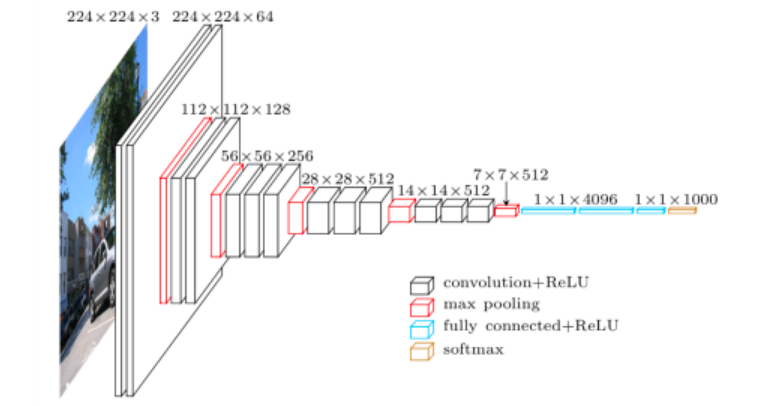
\includegraphics[height = 2.0in]{../images/VGG}}

Each box is a tensor $L[b,x,y,i]$
\begin{eqnarray*}
 & &  L_{\mathrm{out}}[b,x,y,j] \\
 & = & \sigma\left(\left(\sum_{\Delta x, \Delta y, i}\;W[\Delta x, \Delta y, i,j]\; L_{\mathrm{in}}[b,x + \Delta x, y + \Delta y, i]\right) - B[j]\right)
\end{eqnarray*}

\vfill
Each $L_{\mathrm{out}}[b,x,y,j]$ is the output of a single linear threshold unit.

\slide{Padding}

\centerline{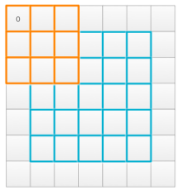
\includegraphics[height = 2.0in]{../images/padding2}}
\centerline{\large Jonathan Hui}

\vfill
If we pad the input with zeros then the input and output can have the same spatial dimensions.

\slide{Zero Padding in NumPy}

In NumPy we can add a zero padding of width p to an image as follows:

\vfill
\begin{verbatim}
padded = np.zeros(W + 2*p,  H + 2*p)

padded[p:W+p, p:H+p] = x
\end{verbatim}

\slide{Padding}

{\tt Procedure CONV}$(\Phi,\; L_{\mathrm{in}}[b,x,y,i],\;\mathrm{padding}\;p)$

\vfill
$L'_{\mathrm{in}} = \mathrm{Padd}(L_{\mathrm{in}},\;p)$

\vfill
$L_{\mathrm{out}}[b,x,y,j] =$

\vfill
$\;\;\;\sigma\left(\left(\sum_{\Delta x, \Delta y, i}\;W[\Delta x, \Delta y, i,j]\;L'_{\mathrm{in}}[b,x + \Delta x, y + \Delta y, i]\right) - B[j] \right)$


\vfill
Return $L_{\mathrm{out}}[b,x,y,j]$

\slide{Reducing Spatial Dimention}

\centerline{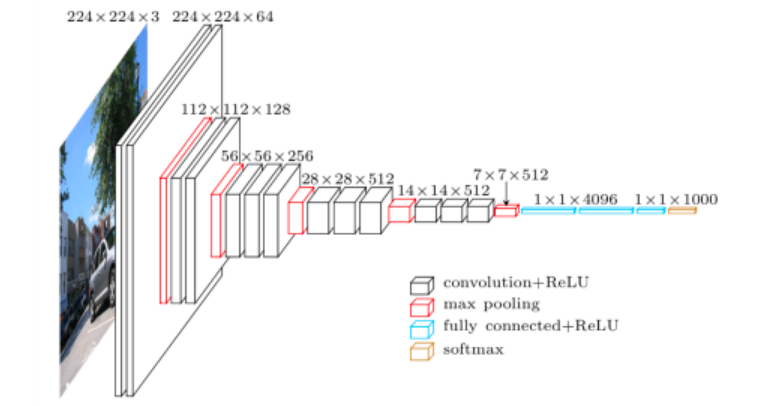
\includegraphics[width = 8.0in]{../images/VGG}}

\slide{Strides}

We can move the filter by a ``stride'' $s$ for each spatial step.

\vfill
$L_{\mathrm{out}}[b,{\color{red}x},{\color{red}y},j] =$

$$\hspace{-1em}\sigma\left(\left(\sum_{\Delta x,\Delta y,i}\;W[\Delta x, \Delta y, i, j] L_{\mathrm{in}}[b,{\color{red} s*x} + \Delta x, {\color{red} s*y} + \Delta y, i]\right) - B[j]\right)$$

\vfill
For strides greater than 1 the spatial dimention is reduced.

\slide{Max Pooling}

$$L_{\mathrm{out}}[b,{\color{red}x},{\color{red}y},i] = {\color{red} \max_{\Delta x, \Delta y}}\; L_{\mathrm{in}}[b,{\color{red} s*x} + \Delta x,\; {\color{red} s*y} + \Delta y,\; i]$$

\vfill
This is typically done with a stride greater than one so that the image dimension is reduced.


\slide{Fully Connected (FC) Layers}

\centerline{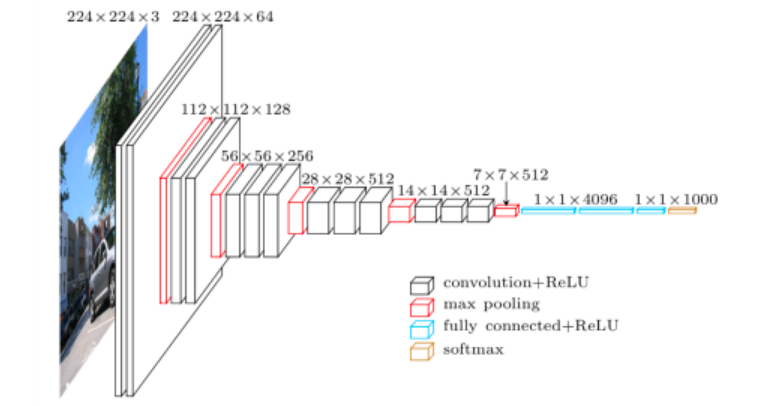
\includegraphics[width = 8.0in]{../images/VGG}}


\slide{Fully Connected (FC) Layers}

We reshape $L_{\mathrm{in}}[b,x,y,i]$ to $L_{\mathrm{in}}[b,i']$ and then

\vfill
$$L_{\mathrm{out}}[b,j] = \sigma\left(\left(\sum_{i'} \;W[j,i']\;L_{\mathrm{in}}[b,i']\right) - B[j]\right)$$

\slide{Alexnet}
{\huge
\centerline{Given Input$[227,227,3]$}

\begin{eqnarray*}
L_1[55 \times 55 \times 96] & = & \relu(\conv(\mathrm{Input},\Phi_1,\mathrm{width}\;11,\pad\;0,\stride\;4)) \\
L_2[27 \times 27 \times 96] & = & \mathrm{MaxPool}(L_1,\mathrm{width}\;3,\stride\;2))  \\
L_3[27 \times 27 \times 256] & = & \relu(\conv(L_2,\Phi_3,\mathrm{width}\;5,\pad\;2,\stride\;1))  \\
L_4[13 \times 13 \times 256] & = & \mathrm{MaxPool}(L_3,\mathrm{width}\;3,\stride\;2))  \\
L_5[13 \times 13 \times 384] & = & \relu(\conv(L_4,\Phi_5,\mathrm{width}\;3,\pad\;1,\stride\;1))  \\
L_6[13 \times 13 \times 384] & = & \relu(\conv(L_5,\Phi_6,\mathrm{width}\;3,\pad\;1,\stride\;1))  \\
L_7[13 \times 13 \times 256] & = & \relu(\conv(L_6,\Phi_7,\mathrm{width}\;3,\pad\;1,\stride\;1))  \\
L_8[6 \times 6 \times 256] & = & \mathrm{MaxPool}(L_7,\mathrm{width}\;3,\stride\;2)) \\
L_9[4096] & = & \relu(\mathrm{FC}(L_8,\Phi_9)) \\
L_{10}[4096] & = & \relu(\mathrm{FC}(L_9,\Phi_{10})) \\
s[1000] & = & \relu(\mathrm{FC}(L_{10},\Phi_s)) \;\;\mbox{class scores}
\end{eqnarray*}
}

\slideplain{VGG, Zisserman, 2014}

\centerline{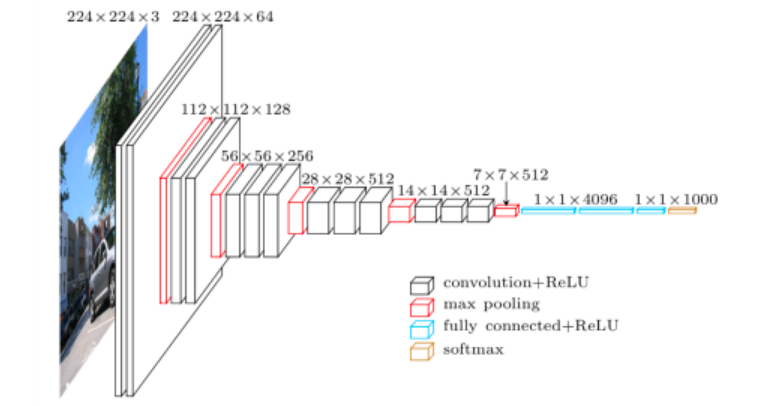
\includegraphics[width = 9.0in]{../images/VGG}}
\centerline{\large Davi Frossard}

\slide{VGG}
\centerline{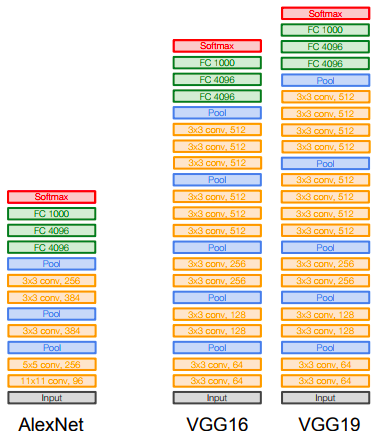
\includegraphics[height=4.5in]{../images/VGGStack}}
\centerline{\large Stanford CS231}

\slide{Inception, Google, 2014}

\centerline{\includegraphics[width = 9.0in]{../images/inception1}}
\vfill
\centerline{\includegraphics[width = 3.5in]{../images/inception2}}

\slide{Imagenet Classification}

1000 kinds of objects.

\vfill
\centerline{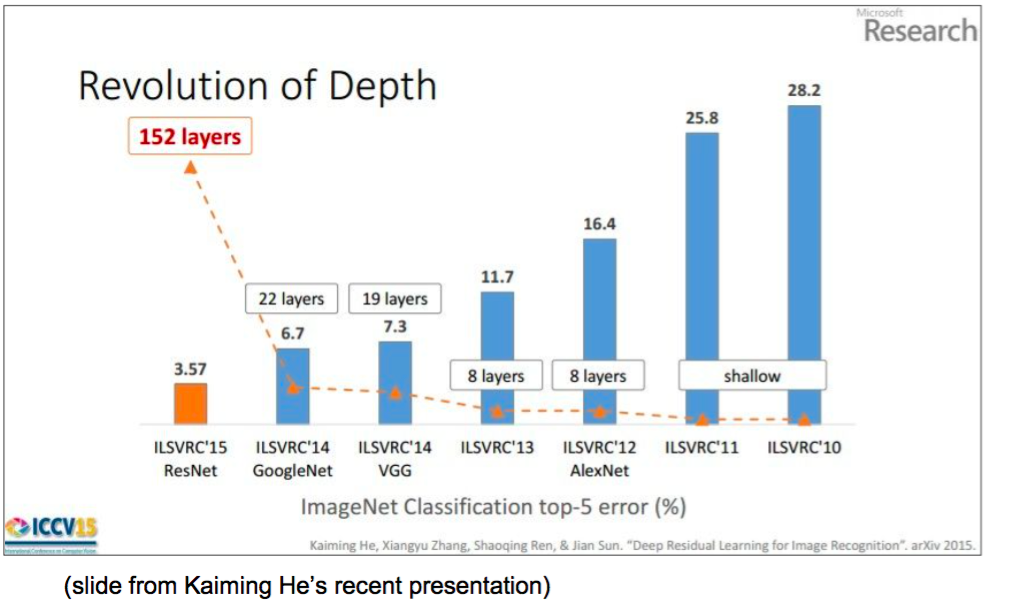
\includegraphics[height=4.5in]{../images/IVLSRC}}
2016 error rate is 3.0\% \hspace{1.0in} 2017 error rate is 2.25\%

\slideplain{Review of The Swap Rule}
\vspace{-3ex}
\begin{eqnarray*}
  {\color{red} \tilde{y}[b,j]} & {\color{red}  =} & {\color{red} \sum_i\;W[j,i]\;x[b,i]} \\
  \\
  y[b,j] & = & \sigma(\tilde{y}[b,j] - B[j]) \\
  \end{eqnarray*}

\vspace{-5ex}
{\color{red} 
  \begin{eqnarray*}
  \\
  x.\mathrm{grad}[b,i] & \pluseq & \sum_j\;\tilde{y}.\mathrm{grad}[b,j]W[j,i] \\
  \\
  W.\mathrm{grad}[j,i] & \pluseq & \sum_b\;\tilde{y}.\mathrm{grad}[b,j]x[b,i]
\end{eqnarray*}
}

\slide{Alternative Swap Rule}
Intialize all computed tensors to zero and write the program using only $\pluseq$.

$$
\begin{array}{lrcl}
{\color{red} \mathrm{for}\;b,i,j} & \tilde{y}[b,j] & \pluseq & W[j,i]\;x[b,i] \\
  \\
{\color{red} \mathrm{for}\;b,i,j} &  x.\mathrm{grad}[b,i] & \pluseq & \tilde{y}.\mathrm{grad}[b,j]W[j,i] \\
  \\
{\color{red} \mathrm{for}\;b,i,j} &  W.\mathrm{grad}[j,i] & \pluseq & \tilde{y}.\mathrm{grad}[b,j]x[b,i]
\end{array}
$$

\vfill
one swaps the output with one of the inputs inside the body of the loop.

\slide{Alternative Swap Rule for Convolution}

\vfill
{\color{red} $\mathrm{for}\;b,x,y,i,j,\Delta x, \Delta y$}
$$\tilde{L}_{\mathrm{out}}[b,x,y,j] \;\pluseq\; W[\Delta x, \Delta y, i, j]\;L_{\mathrm{in}}[b,x + \Delta x, y + \Delta y, i]$$

\vfill
{\color{red} $\mathrm{for}\;b,x,y,i,j,\Delta x, \Delta y$ }
$$\;\;\;W.\mathrm{grad}[\Delta x, \Delta y,i,j] \; \pluseq \; \tilde{L}_{\mathrm{out}}.\grad[b,x,y,j]\;L_{\mathrm{in}}[b,x + \Delta x,y+ \Delta y,i]$$

\vfill
{\color{red} $\mathrm{for}\;b,x,y,i,j,\Delta x, \Delta y$}
$$\;{\color{red} L_{\mathrm{in}}.\grad[b,x+\Delta x,y+\Delta y,i,j]} \;\pluseq \; \tilde{L}_{\mathrm{out}}.\grad[b,x,y,j]\;W[\Delta x, \Delta y, i, j]$$


\slide{Image to Column (Im2C)}

Reduce convolution to matrix multiplication ---  more space but faster.
{\huge
  $$L_{\mathrm{in}}[b,x,y,\Delta x,\Delta y,i] = L_{\mathrm{in}}[b,x+\Delta x,y+\Delta y,i]$$

\begin{eqnarray*}
  & & \tilde{L}_{\mathrm{out}}[b,x,y,j] \\
  \\
  & = & \left(\sum_{\Delta x, \Delta y, i} W[\Delta x, \Delta y, i, j] *L_{\mathrm{in}}[b,x + \Delta x,\; y + \Delta y,\; i]\right) + B[j] \\
  \\
      & = & \left(\sum_{\Delta x, \Delta y, i} \begin{array}{l}
                                              L_{\mathrm{in}}[b,x,y,\Delta x,\Delta y,i]
                                              * W[\Delta x, \Delta y, i, j] \\
  \end{array}\right) + B[j] \\
  \\
    & = & \left(\sum_{(\Delta x, \Delta y, i)} \begin{array}{l}
                                              L_{\mathrm{in}}[(b,x,y),(\Delta x,\Delta y,i)]
                                              * W[(\Delta x, \Delta y, i), j] \\
                                           \end{array}\right) + B[j]
\end{eqnarray*}
}

\slideplain{Fully Convolutional Networks}

\centerline{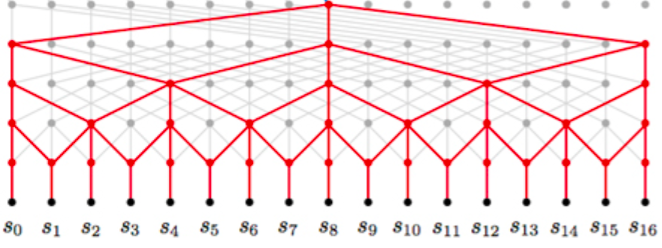
\includegraphics[width=8.0in]{../images/dilation}}

\slide{Dilation}

We can ``dilate'' the filter by introducing an image step size $d$ for each step in the filter coordinates.

\vfill
\begin{eqnarray*}
\tilde{L}_{\mathrm{out}}[b,x,y,j] & = &  W[\Delta x, \Delta y, i, j] L_{\mathrm{in}}[b,x + {\color{red} d*\Delta x}, y + {\color{red} d*\Delta y}, i] + B[j]
\end{eqnarray*}

This is used for ``fully convolutional'' CNNs.


\slide{Summary}

\begin{itemize}
\item Convolution

\vfill
\item Padding

  \vfill
\item Stides

  \vfill
\item Max Pooling

  \vfill
\item Fully Connected Layers

  \vfill
\item Dilation
\end{itemize}

\slide{Modern Trends}

Modern Convolutions use 3X3 filters.  This is faster and has fewer parameters.  Expressive power is preserved by increasing depth with many stride 1 layers.

\vfill
Max pooling and dilation seem to have disappeared.

\vfill
Resnet and resnet-like architectures are now dominant (next lecture).


\slideplain{END}

}
\end{document}
